\documentclass[conference,a4paper]{IEEEtran}

\usepackage[utf8]{inputenc}
\usepackage[T1]{fontenc}
\usepackage[spanish,es-noshorthands,es-tabla,es-nodecimaldot]{babel}
\usepackage{newtxtext,newtxmath}
\usepackage{graphicx}
\usepackage{booktabs}
\usepackage{array}
\usepackage{multirow}
\usepackage[table]{xcolor}
\usepackage[nocompress]{cite}
\usepackage{amsmath}
\usepackage{caption}
\usepackage{subcaption}
\usepackage{stfloats}
\usepackage{tikz}
\usetikzlibrary{arrows.meta,positioning,shapes.geometric,fit,calc,backgrounds}
\usepackage{url}
\usepackage[hidelinks]{hyperref}

% Sin guiones de corte al final de línea
\hyphenpenalty=10000
\exhyphenpenalty=10000
\emergencystretch=3em

% Subsecciones numeradas como A, B, C sin guion
\renewcommand{\thesubsection}{\Alph{subsection}}
\renewcommand{\thesubsubsection}{\arabic{subsubsection}}

% Marca en rojo lo que el equipo debe completar con sus mediciones
\newcommand{\pend}[1]{\textcolor{red}{\textbf{[#1]}}}

\captionsetup[subfigure]{font=footnotesize,labelfont=footnotesize}
\graphicspath{{figuras/}}

\definecolor{azul}{HTML}{1F4E79}
\definecolor{azulclaro}{HTML}{DCE8F4}
\definecolor{naranja}{HTML}{D9822B}
\definecolor{naranjaclaro}{HTML}{FBE7D3}
\definecolor{verde}{HTML}{2E7D32}
\definecolor{verdeclaro}{HTML}{DFF0E0}
\definecolor{grisclaro}{HTML}{EFEFEF}
\definecolor{rojo}{HTML}{B22222}

\tikzset{
  bloque/.style={draw, rounded corners=2pt, align=center, font=\scriptsize, inner sep=3pt, minimum height=7mm},
  sensor/.style={bloque, fill=azulclaro, text width=24mm},
  actuador/.style={bloque, fill=naranjaclaro, text width=24mm},
  red/.style={bloque, fill=verdeclaro, text width=24mm},
  flecha/.style={-{Stealth[length=2mm]}, thick},
  doble/.style={{Stealth[length=2mm]}-{Stealth[length=2mm]}, thick},
  proceso/.style={draw, fill=azulclaro, rounded corners=1pt, align=center, font=\scriptsize, text width=30mm, minimum height=6mm, inner sep=2pt},
  decision/.style={draw, fill=naranjaclaro, diamond, aspect=2.6, align=center, font=\scriptsize, inner sep=0.5pt, text width=21mm},
  terminal/.style={draw, fill=grisclaro, rounded corners=3mm, align=center, font=\scriptsize, minimum height=6mm, text width=22mm},
  alerta/.style={draw, fill=red!12, rounded corners=1pt, align=center, font=\scriptsize, text width=30mm, minimum height=6mm, inner sep=2pt},
  es/.style={draw, fill=verdeclaro, trapezium, trapezium left angle=72, trapezium right angle=108, trapezium stretches body, align=center, font=\scriptsize, text width=27mm, minimum height=6mm, inner sep=1.5pt},
  potencia/.style={-{Stealth[length=2mm]}, line width=1.4pt, rojo},
  interfaz/.style={font=\tiny, above, inner sep=1pt},
}

\begin{document}

\title{SafeCane: bastón inteligente IoT para detectar obstáculos, desniveles y caídas en personas con discapacidad visual y adultos mayores}

\author{\IEEEauthorblockN{Nayeli Fernanda Guzman Huayta, Jazmin Nicole Soto Quiñones y Manyory Estefany Cueva Mendoza}
\IEEEauthorblockA{CS5055: Internet of Things\\
Universidad de Ingeniería y Tecnología (UTEC)\\
Lima, Perú}}

\maketitle

% =====================================================================
\section{Introducción, problemática y marco teórico}

\subsection{Introducción}

\IEEEPARstart{E}{l} Internet de las Cosas (IoT) conecta objetos de uso diario que tienen sensores, capacidad de cálculo y comunicación, de modo que pueden intercambiar datos entre ellos y con servicios en la nube sin que una persona intervenga en cada paso \cite{atzori}. En salud y asistencia esta idea se conoce como Ambient Assisted Living (AAL): dispositivos que acompañan a personas mayores o con discapacidad y avisan a un familiar o cuidador cuando ocurre algo que pone en riesgo a la persona \cite{tsantikidou}.

El bastón blanco sigue siendo la ayuda de movilidad más usada por las personas con discapacidad visual porque es barato y fácil de usar. Su problema es que solo informa de lo que toca la punta. Desde hace años se proponen ayudas electrónicas de desplazamiento (Electronic Travel Aids, ETA) que suman sensores ultrasónicos, infrarrojos o cámaras para ampliar ese alcance \cite{dakopoulos}. Hoy, con microcontroladores baratos que traen WiFi y Bluetooth integrados, también es posible añadir detección de caídas, ubicación y aviso remoto en el mismo bastón.

Este informe presenta SafeCane, un bastón inteligente pensado para personas con discapacidad visual y para adultos mayores, dos grupos cuyas necesidades al caminar se parecen mucho. El bastón mide la distancia a los obstáculos que tiene al frente con un sensor ultrasónico HC-SR04, detecta escalones que bajan o bordillos con un sensor infrarrojo FC-51 ubicado cerca de la punta, reconoce caídas con una unidad inercial MPU6050 y guarda la posición del módulo GPS NEO-6M cuando se genera una alerta. Un ESP32 procesa todo dentro del bastón, avisa al usuario con vibración y sonido, y envía el estado y las alertas por Bluetooth de baja energía a un celular y por MQTT a un tablero web.

Para los desniveles elegimos el FC-51 porque el ultrasonido no detecta lo que pasa bajo la punta, y un escalón que baja es justo el tipo de obstáculo que provoca caídas. El bastón deduce si está en uso a partir del movimiento que registra la unidad inercial.

\subsection{Problemática}

La Organización Mundial de la Salud (OMS) estima que al menos 2\,200 millones de personas tienen algún deterioro de la visión cercana o lejana, y que en al menos 1\,000 millones de esos casos el problema pudo prevenirse o todavía no ha sido atendido \cite{oms_vision}. En el Perú, el Instituto Nacional de Estadística e Informática (INEI) registró 3\,209\,261 personas con alguna discapacidad, el 10,3\,\% de la población. De ellas, 1\,550\,196 (48,3\,\%) declararon dificultad para ver aun usando anteojos, lo que convierte a la discapacidad visual en la más frecuente del país. Además, la prevalencia crece con la edad y llega a sus valores más altos a partir de los 60 años \cite{inei}.

Ese grupo de mayor edad es también el que más sufre con las caídas. La OMS estimó unas 842\,000 muertes por caídas en 2023, lo que las ubica como la segunda causa de muerte por lesiones no intencionales en el mundo, después de los accidentes de tránsito. Cerca del 71\,\% de esas muertes ocurrió en personas de 60 años o más \cite{oms_caidas}. La relación entre visión y caídas está documentada: una revisión de la literatura concluyó que las personas con discapacidad visual se caen y se lesionan más que la población general \cite{legood}. Appiah y Elmannai citan que cerca del 30\,\% de los adultos mayores de 65 años se cae cada año y que ese riesgo es más del doble en quienes tienen discapacidad visual \cite{appiah}.

El bastón blanco tiene tres limitaciones. No anticipa obstáculos que están más arriba del suelo ni avisa de un escalón que baja \cite{dakopoulos}, \cite{paredes}. No registra si la persona se cae, así que quien camina solo puede quedarse en el suelo mucho tiempo antes de que alguien lo note, y esa demora empeora la lesión \cite{fitriandini}. Por último, no permite saber dónde está la persona si se desorienta o necesita ayuda \cite{abuelmakarem}. Falta un dispositivo de bajo costo que amplíe la detección, reconozca una caída, registre dónde ocurrió y avise a la familia. Con SafeCane buscamos acortar el tiempo que pasa entre la caída y la llegada de ayuda.

\subsection{Marco teórico}

\subsubsection{IoT y Ambient Assisted Living}
Atzori et al. \cite{atzori} describen una arquitectura IoT en tres capas. La capa de percepción contiene los sensores y actuadores, la capa de red transporta los datos y la capa de aplicación ofrece los servicios que usan esa información. SafeCane sigue esa estructura. El bastón es la capa de percepción, BLE y WiFi forman la capa de red, y el celular junto con el tablero web son la capa de aplicación. Un sistema AAL acorta el tiempo entre un evento adverso y la respuesta del cuidador, y guarda un registro de lo ocurrido \cite{tsantikidou}.

\subsubsection{Medición de distancia por ultrasonido}
El HC-SR04 emite un tren de pulsos de 40\,kHz y mide el tiempo $t$ que tarda en volver el eco. Con la velocidad del sonido en el aire, $v \approx 343$\,m/s, la distancia es
\begin{equation}
d = \frac{v \cdot t}{2},
\label{eq:distancia}
\end{equation}
donde el factor 2 corrige el viaje de ida y vuelta. El haz forma un cono de unos 15°. Las superficies duras y planas reflejan bien la onda, mientras que la tela, el vidrio o las superficies inclinadas pueden absorberla o desviarla \cite{abuelmakarem}.

\subsubsection{Detección de caídas con una unidad inercial}
El MPU6050 tiene un acelerómetro y un giroscopio de tres ejes \cite{mpu6050}. Con las aceleraciones $a_x$, $a_y$ y $a_z$ se calcula la magnitud del vector de aceleración, conocida como SVM:
\begin{equation}
\mathrm{SVM} = \sqrt{a_x^2 + a_y^2 + a_z^2}.
\label{eq:svm}
\end{equation}
En reposo la SVM vale cerca de 1\,g. Una caída suele tener tres fases: una caída libre breve en la que la SVM baja de 1\,g, un impacto que supera varias veces la gravedad y un periodo final de quietud con otra orientación. Bourke et al. \cite{bourke} mostraron que combinar un umbral inferior para la caída libre con uno superior para el impacto distingue caídas de actividades diarias mejor que un solo umbral. La inclinación del bastón respecto de la vertical se obtiene como $\theta = \arccos(a_z/\mathrm{SVM})$.

\subsubsection{Detección de desniveles por reflexión infrarroja}
El FC-51 tiene un LED infrarrojo, un fotodiodo y un comparador LM393 que se ajusta con un potenciómetro. El módulo compara la luz que rebota con un umbral, sin medir distancia, y su salida es baja cuando ve el piso y alta cuando deja de verlo. Si el sensor va cerca de la punta mirando hacia abajo, un cambio a nivel alto significa que el piso «desapareció» delante del bastón, como ocurre al llegar a un escalón que baja o a un bordillo. Su alcance depende del color del piso y la luz solar directa puede cegarlo.

\subsubsection{Ubicación y comunicación}
El receptor GPS calcula latitud y longitud con las señales de cuatro o más satélites y entrega los datos por puerto serie en frases NMEA. El NEO-6M ofrece una precisión horizontal de unos 2,5\,m CEP y tarda alrededor de 27\,s en un arranque en frío \cite{neo6m}. Para la comunicación se usan dos canales. BLE conecta el bastón con un celular cercano con poco consumo. WiFi permite publicar los datos con MQTT, un protocolo ligero de publicación y suscripción en el que los dispositivos envían mensajes a tópicos de un intermediario (broker) y los clientes interesados se suscriben a esos tópicos \cite{mqtt}.

% =====================================================================
\section{Estado del arte}

Para esta revisión cada integrante analizó dos artículos de los últimos siete años y luego sumamos dos trabajos sobre detección de caídas en bastones que fueron clave para el algoritmo. Los agrupamos en tres líneas: bastones con detección de obstáculos y conectividad, detección de caídas con unidades inerciales, y bastones para el monitoreo de adultos mayores. La Tabla~\ref{tab:comparacion} resume la comparación.

\subsection{Bastones con detección de obstáculos y conectividad}

Paredes Orozco y Domínguez-Morales \cite{paredes} desarrollaron en la Universidad de Sevilla un bastón que detecta obstáculos a mayor distancia que el bastón blanco y también a la altura del torso, con ángulos de detección más amplios en vertical y horizontal. El bastón se acompaña de una aplicación móvil que guía al usuario, sigue su ubicación y ofrece asistencia de emergencia, e incluye detección de caídas con envío de coordenadas GPS a la familia. Los autores reportan cerca de 98\,\% de exactitud en obstáculos y casi 50 horas de autonomía. Es el trabajo más completo de la revisión y demuestra que obstáculos, caídas y GPS caben en un mismo bastón. Sin embargo, no detalla el microcontrolador ni trata los desniveles bajo la punta, y su autonomía queda como referencia difícil de alcanzar para un prototipo con GPS encendido todo el tiempo.

Abuelmakarem et al. \cite{abuelmakarem} proponen un bastón con cinco sensores ultrasónicos que cubren 180° y detectan escaleras, un sensor de agua para charcos, un sensor de llama y una LDR que enciende LEDs en la oscuridad. Un Arduino Uno procesa los sensores y reproduce mensajes de audio, y un NodeMCU (ESP8266) envía la ubicación a la plataforma Blynk. Al calibrar los sensores encontraron que la lectura cambia según el material del obstáculo, con diferencias entre madera, vidrio y concreto. En SafeCane asumimos la misma limitación del ultrasonido. Su arquitectura de dos microcontroladores, en cambio, nos convenció de usar un solo ESP32 que ya trae WiFi y Bluetooth.

Tsantikidou et al. \cite{tsantikidou} diseñaron un bastón basado en el paradigma AAL que detecta obstáculos a nivel del suelo y de la cabeza con ultrasonido y vibración, reconoce escaleras con visión por computador y tiene un botón de emergencia. Se comunica por LoRa con cifrado y mecanismos de privacidad, sobre un Arduino Nano y una Raspberry Pi Zero. Reportan una mejora de 7,4\,\% en la exactitud de detección de obstáculos frente a sistemas parecidos y una detección de escaleras sin errores. De este trabajo tomamos dos ideas: la vibración como canal principal de aviso y el cuidado de la ubicación como dato sensible. Por la segunda usamos un tópico MQTT propio y dejamos prevista la opción de un broker con autenticación.

\subsection{Detección de caídas con unidades inerciales}

Fitriandini et al. \cite{fitriandini} construyeron un detector de caídas para adultos mayores con dos de los sensores que usa SafeCane: el acelerómetro MPU-6050 y el GPS NEO-6M. Cuando detectan una caída suena un zumbador y llega una notificación a una aplicación Android que muestra la posición en Google Maps. Midieron un error de ubicación de 3,47\,m en el eje x, 3,07\,m en el eje y y 4,63\,m radial, con un retardo medio de notificación de 4,71\,s. Es el antecedente más cercano al proyecto, porque valida la combinación MPU6050, NEO-6M y alarma sonora, y nos da dos cifras para comparar nuestras pruebas: el error de ubicación y la latencia de la alerta.

Appiah y Elmannai \cite{appiah} integran en un bastón blanco la detección de caídas y la detección de obstáculos por ultrasonido con retroalimentación háptica. Cuando el bastón detecta una caída envía un mensaje de texto a los familiares o al personal indicado, y los autores reportan más de 95\,\% de exactitud en la detección. Su propuesta confirma que juntar obstáculos y caídas en un solo dispositivo es viable con hardware sencillo, aunque depende de la red celular para avisar.

Geng et al. \cite{geng} atacan el problema más difícil de un bastón con detector de caídas: el bastón golpea el piso muchas veces por minuto y puede caerse sin que el usuario se caiga. Su bastón usa un ESP32-S3, un MPU6050 y un sensor MAX30102 de frecuencia cardiaca y oxígeno. Combinan umbrales en varios niveles sobre el ángulo de actitud, la aceleración y las señales fisiológicas con un mecanismo de confirmación interactiva, y reportan 97,2\,\% de exactitud en 500 acciones simuladas. De este trabajo sale la ventana de cancelación de 10\,s de SafeCane.

Shri Harini et al. \cite{shriharini} usan un perceptrón multicapa con activación ReLU para analizar los datos de un MPU6050 y reconocer patrones de movimiento, cambios de orientación y caídas, además de detectar obstáculos. El sistema avisa a los cuidadores mediante una base de datos en la nube y correo electrónico. Para esta etapa elegimos umbrales porque son fáciles de explicar y de ajustar. Los datos que registramos durante las pruebas servirán para entrenar un clasificador más adelante.

\subsection{Bastones para el monitoreo de adultos mayores}

Putera et al. \cite{putera} desarrollaron en Batam, Indonesia, un bastón para adultos mayores con sensores de frecuencia cardiaca y oxígeno en sangre (MAX30102), temperatura (MLX90614), un sensor no invasivo de glucosa, GPS, una minicámara con audio y un panel solar, todo controlado por un ESP32 conectado a Blynk. Midieron una precisión GPS de 3 a 5\,m contra Google Maps, pero la saturación de oxígeno promedio (89\,\%) quedó por debajo de la norma clínica. El trabajo confirma que el ESP32 basta para un bastón con GPS y monitoreo remoto. También deja ver que los sensores biomédicos exigen una validación médica que está fuera de nuestro alcance, y por eso limitamos SafeCane a la movilidad y las caídas.

\subsection{Síntesis}

Ninguno de los trabajos revisados reúne en un dispositivo de bajo costo la detección de obstáculos al frente, el aviso de desniveles bajo la punta, la detección de caídas y la ubicación de cada alerta. Los desniveles son la función menos cubierta, ya que solo \cite{tsantikidou} y \cite{abuelmakarem} detectan escaleras y lo hacen con cámara o con varios ultrasonidos. El riesgo técnico de nuestra propuesta es moderado porque la pareja MPU6050 y NEO-6M ya tiene validación experimental \cite{fitriandini} y el ESP32 funciona bien en un bastón parecido \cite{putera}.

\begin{table*}[!t]
\caption{Comparación de los trabajos revisados con SafeCane}
\label{tab:comparacion}
\centering
\scriptsize
\renewcommand{\arraystretch}{1.2}
\setlength{\tabcolsep}{3.5pt}
\begin{tabular}{>{\raggedright\arraybackslash}p{2.6cm} >{\raggedright\arraybackslash}p{3.3cm} >{\raggedright\arraybackslash}p{2.2cm} >{\raggedright\arraybackslash}p{2.0cm} c c c >{\raggedright\arraybackslash}p{2.6cm}}
\toprule
\textbf{Estudio} & \textbf{Sensores principales} & \textbf{Controlador} & \textbf{Comunicación} & \textbf{Obst.} & \textbf{Desniv.} & \textbf{Caídas / GPS} & \textbf{Resultado clave} \\
\midrule
Paredes Orozco y D.\ M. \cite{paredes} (2024) & Obstáculos en suelo y torso, IMU, GPS & No especificado & App móvil & Sí & No & Sí / Sí & 98\,\% de exactitud, 50\,h de batería \\
Tsantikidou et al. \cite{tsantikidou} (2025) & Ultrasonido en suelo y cabeza, cámara, botón SOS & Arduino Nano y Raspberry Pi Zero & LoRa cifrado & Sí & Escaleras & No / No & 7,4\,\% más de exactitud \\
Fitriandini et al. \cite{fitriandini} (2025) & MPU-6050, GPS NEO-6M, zumbador & Tipo Arduino & WiFi, app Android & No & No & Sí / Sí & 4,63\,m de error y 4,71\,s de latencia \\
Abuelmakarem et al. \cite{abuelmakarem} (2024) & Cinco ultrasonidos, agua, llama, LDR & Arduino Uno y NodeMCU & WiFi, Blynk & Sí & Escaleras & No / Sí & Cobertura de 180° \\
Appiah y Elmannai \cite{appiah} (2023) & Ultrasonido, sensor de caídas, vibración & No especificado & SMS & Sí & No & Sí / No reportado & Más de 95\,\% de exactitud en caídas \\
Geng et al. \cite{geng} (2026) & MPU-6050, MAX30102 & ESP32-S3 & No reportado & No & No & Sí / No & 97,2\,\% de exactitud en 500 pruebas \\
Putera et al. \cite{putera} (2025) & MAX30102, MLX90614, glucosa, GPS, cámara & ESP32 & WiFi, Blynk & No & No & No / Sí & GPS de 3 a 5\,m \\
Shri Harini et al. \cite{shriharini} (2026) & MPU6050, obstáculos & Embebido de bajo consumo & Nube y correo & Sí & No & Sí / No & Caídas clasificadas con MLP \\
\midrule
\textbf{SafeCane} & HC-SR04, FC-51, MPU6050, NEO-6M & ESP32 & BLE, WiFi y MQTT & Sí & Sí & Sí / Sí & Reúne las cuatro funciones \\
\bottomrule
\end{tabular}
\end{table*}

% =====================================================================
\section{Metodología y desarrollo del proyecto}

\subsection{Enfoque de trabajo}

Trabajamos con prototipado incremental. Probamos cada sensor por separado antes de juntarlo con los demás, y no pasamos a la fase siguiente hasta cumplir los criterios de la anterior. La Tabla~\ref{tab:fases} muestra las etapas. Desde la Fase 3 usamos un único firmware, y entre etapas solo cambian tres banderas al inicio del código: red activa, medición de batería y modo de registro de datos.

\begin{table}[!t]
\caption{Etapas del desarrollo}
\label{tab:fases}
\centering
\footnotesize
\renewcommand{\arraystretch}{1.15}
\begin{tabular}{c p{6.6cm}}
\toprule
\textbf{Fase} & \textbf{Qué se hizo} \\
\midrule
0 & Entorno de programación en Arduino IDE con el núcleo ESP32 \\
1 & Prueba de cada sensor y actuador por separado \\
2 & Integración eléctrica en protoboard \\
3 & Firmware integrado con máquina de estados, sin red \\
4 & Registro de datos a 50\,Hz para calibrar los umbrales \\
5 & Comunicación por WiFi, MQTT y BLE, y tablero web \\
6 & Alimentación autónoma con batería \\
7 & Montaje del circuito en el bastón \\
8 & Validación final con pruebas \\
\bottomrule
\end{tabular}
\end{table}

\subsection{Planteamiento del sistema}

La Fig.~\ref{fig:bloques} presenta el sistema en bloques. A la izquierda están las entradas: el HC-SR04 mira al frente, el FC-51 mira al piso, el MPU6050 mide aceleración e inclinación, el NEO-6M entrega la posición y el pulsador permite cancelar una alerta. En el centro, el ESP32 reparte el trabajo entre sus dos núcleos. El núcleo 1 lee los sensores y toma las decisiones, y el núcleo 0 se ocupa solo de la red. Esta separación hace que la alerta local nunca dependa del WiFi: si se pierde la conexión, el bastón sigue vibrando y sonando. A la derecha están los actuadores y abajo la comunicación hacia el celular y el tablero.

\begin{figure*}[!t]
\centering
\begin{tikzpicture}[node distance=2.2mm and 9mm]
  % Entradas
  \node[sensor] (hc) {\textbf{HC-SR04}\\obstáculos al frente};
  \node[sensor, below=of hc] (fc) {\textbf{FC-51}\\desnivel bajo la punta};
  \node[sensor, below=of fc] (mpu) {\textbf{MPU6050}\\caídas e inclinación};
  \node[sensor, below=of mpu] (gps) {\textbf{GPS NEO-6M}\\ubicación};
  \node[sensor, below=of gps] (btn) {\textbf{Pulsador}\\cancelar alerta};
  \node[font=\scriptsize\bfseries, above=1mm of hc] {ENTRADAS};

  % ESP32
  \node[bloque, fill=white, text width=46mm, right=13mm of hc.north east, anchor=north west, minimum height=8mm] (n1)
    {\textbf{Núcleo 1: sensores y decisiones}\\FC-51 cada 10\,ms, IMU a 50\,Hz\\distancia cada 100\,ms\\algoritmo de caída y máquina de estados\\control del motor y el buzzer};
  \node[bloque, fill=white, text width=46mm, below=4mm of n1] (n0)
    {\textbf{Núcleo 0: comunicación}\\conexión WiFi y MQTT con reintentos\\tópicos de estado, alerta y GPS\\notificaciones BLE};
  \begin{scope}[on background layer]
    \node[draw, thick, rounded corners=3pt, fill=grisclaro, fit=(n1)(n0)(n1.north |- hc.north)(n0.south |- btn.south), inner sep=3mm, label={[font=\scriptsize\bfseries]above:ESP32-WROOM-32}] (esp) {};
  \end{scope}

  % Salidas
  \node[actuador, right=13mm of n1.north east, anchor=north west] (mot) {\textbf{Motor vibrador}\\aviso háptico por PWM};
  \node[actuador, below=of mot] (buz) {\textbf{Buzzer activo}\\desnivel y alarma};
  \node[font=\scriptsize\bfseries, above=1mm of mot] {SALIDAS};

  % Comunicación
  \node[red, below=10mm of buz] (cel) {\textbf{Celular cercano}\\estado y alertas};
  \node[red, below=of cel] (broker) {\textbf{Broker MQTT}\\estado, alerta, gps};
  \node[red, below=of broker] (tab) {\textbf{Tablero web}\\estado, alertas y mapa};
  \node[font=\scriptsize\bfseries, above=1mm of cel] {COMUNICACIÓN};

  % Flechas entradas
  \draw[flecha] (hc.east) -- node[interfaz]{Digital} (esp.west |- hc.east);
  \draw[flecha] (fc.east) -- node[interfaz]{Digital} (esp.west |- fc.east);
  \draw[flecha] (mpu.east) -- node[interfaz]{I2C} (esp.west |- mpu.east);
  \draw[flecha] (gps.east) -- node[interfaz]{UART} (esp.west |- gps.east);
  \draw[flecha] (btn.east) -- node[interfaz]{Digital} (esp.west |- btn.east);
  % Flechas salidas
  \draw[flecha] (esp.east |- mot.west) -- node[interfaz]{PWM} (mot.west);
  \draw[flecha] (esp.east |- buz.west) -- node[interfaz]{Digital} (buz.west);
  \draw[flecha, verde] (esp.east |- n0.north) -- ++(4mm,0) |- node[pos=0.75, above, font=\tiny]{BLE} (cel.west);
  \draw[flecha, verde] (esp.east |- n0.south) -- ++(8mm,0) |- node[pos=0.75, above, font=\tiny]{WiFi} (broker.west);
  \draw[flecha, verde] (broker) -- node[right, font=\tiny]{WebSocket} (tab);

  % Alimentación
  \path (esp.south |- tab.south) ++(0,-5mm) node[bloque, fill=yellow!15, text width=120mm, anchor=north] (pwr)
    {\textbf{Alimentación:} portapilas doble con dos celdas de litio de 3,7\,V en serie (unos 7,4\,V) $\rightarrow$ pines VIN y GND del ESP32; su regulador interno entrega 3,3\,V};
  \draw[potencia] (pwr.north) -- node[right, font=\tiny, text=rojo]{VIN, unos 7,4\,V} (esp.south);
  % Leyenda
  \coordinate (ley) at ($(pwr.south west)+(0,-4mm)$);
  \draw[flecha] (ley) -- ++(6mm,0) node[right, font=\tiny]{datos};
  \draw[potencia] ($(ley)+(20mm,0)$) -- ++(6mm,0) node[right, font=\tiny, text=black]{potencia};
  \draw[flecha, verde] ($(ley)+(42mm,0)$) -- ++(6mm,0) node[right, font=\tiny, text=black]{inalámbrico};
\end{tikzpicture}
\caption{Diagrama de bloques de SafeCane. Cada flecha de datos indica su interfaz y la línea roja gruesa marca la alimentación. Las entradas llegan al ESP32, que decide en el núcleo 1 y comunica en el núcleo 0. Los actuadores avisan al usuario y la red avisa a la familia.}
\label{fig:bloques}
\end{figure*}

\subsection{Decisiones tomadas a partir del estado del arte}

Tomamos varias decisiones del diseño a partir de los trabajos revisados. La Fig.~\ref{fig:decisiones} las resume y muestra de qué antecedente viene cada una. La más importante es la confirmación antes de enviar la alerta, que tomamos de Geng et al. \cite{geng}, porque en un bastón las falsas alarmas son el principal riesgo. También elegimos la vibración como aviso principal, siguiendo a Dakopoulos y Bourbakis \cite{dakopoulos}, que advierten que el audio tapa los sonidos del entorno de los que depende una persona ciega para orientarse. Por eso el buzzer queda reservado para los desniveles y las caídas.

\begin{figure}[!t]
\centering
\begin{tikzpicture}[
  ant/.style={bloque, fill=azulclaro, text width=27mm, minimum height=9mm},
  dec/.style={bloque, fill=naranjaclaro, text width=40mm, minimum height=9mm},
  node distance=2mm and 6mm]
  \node[ant] (a1) {Geng et al. \cite{geng}\\Appiah y Elmannai \cite{appiah}};
  \node[dec, right=of a1] (d1) {Ventana de 10\,s para cancelar antes de enviar la alerta};
  \node[ant, below=of a1] (a2) {Bourke et al. \cite{bourke}};
  \node[dec, right=of a2] (d2) {Dos umbrales de SVM: caída libre e impacto};
  \node[ant, below=of a2] (a3) {Dakopoulos y Bourbakis \cite{dakopoulos}\\Tsantikidou et al. \cite{tsantikidou}};
  \node[dec, right=of a3] (d3) {Vibración como aviso principal y sonido solo en eventos críticos};
  \node[ant, below=of a3] (a4) {Fitriandini et al. \cite{fitriandini}};
  \node[dec, right=of a4] (d4) {MPU6050 con NEO-6M y metas de 4,63\,m y 4,71\,s};
  \node[ant, below=of a4] (a5) {Abuelmakarem et al. \cite{abuelmakarem}\\Putera et al. \cite{putera}};
  \node[dec, right=of a5] (d5) {Un solo ESP32 con WiFi y BLE integrados};
  \node[ant, below=of a5] (a6) {Tsantikidou et al. \cite{tsantikidou}\\Abuelmakarem et al. \cite{abuelmakarem}};
  \node[dec, right=of a6] (d6) {Desniveles con un sensor infrarrojo barato en lugar de cámara};
  \node[ant, below=of a6] (a7) {Shri Harini et al. \cite{shriharini}};
  \node[dec, right=of a7] (d7) {Umbrales ahora y datos guardados para un clasificador después};
  \foreach \i in {1,...,7} \draw[flecha] (a\i) -- (d\i);
  \node[font=\scriptsize\bfseries, above=1mm of a1] {Antecedente};
  \node[font=\scriptsize\bfseries, above=1mm of d1] {Decisión en SafeCane};
\end{tikzpicture}
\caption{Relación entre los trabajos del estado del arte y las decisiones de diseño de SafeCane.}
\label{fig:decisiones}
\end{figure}

\subsection{Componentes}

La Tabla~\ref{tab:componentes} lista los componentes del prototipo con su función. Elegimos el ESP32-WROOM-32 porque trae WiFi y Bluetooth en el mismo chip, tiene dos núcleos a 240\,MHz, entradas analógicas de 12 bits, I2C y tres puertos serie, uno de los cuales queda libre para el GPS \cite{esp32}. Trabajar a 3,3\,V obliga a dos ajustes en el circuito. La señal Echo del HC-SR04 sale a 5\,V y se baja con un divisor de 1\,k$\Omega$ y 2\,k$\Omega$. El buzzer se conmuta con un transistor 2N2222 porque un pin del ESP32 no entrega la corriente que necesita, y el motor usa un módulo vibrador de 5\,V que ya trae su propio transistor y diodo, así que su entrada va directo al pin.

\begin{table}[!t]
\caption{Componentes del prototipo}
\label{tab:componentes}
\centering
\footnotesize
\renewcommand{\arraystretch}{1.12}
\begin{tabular}{>{\raggedright\arraybackslash}p{2.7cm} >{\raggedright\arraybackslash}p{5.1cm}}
\toprule
\textbf{Componente} & \textbf{Función y dato técnico} \\
\midrule
ESP32-WROOM-32 & Procesamiento y comunicación. Doble núcleo a 240\,MHz, WiFi y Bluetooth 4.2 \cite{esp32} \\
HC-SR04 & Distancia a obstáculos, de 2\,cm a 4\,m, haz de unos 15° \\
FC-51 & Desniveles bajo la punta. Salida digital con comparador LM393 \\
Módulo inercial MPU & Caídas e inclinación. Acelerómetro configurado en $\pm$8\,g \cite{mpu6050} \\
GPS NEO-6M & Ubicación. UART a 9600\,bps, 2,5\,m CEP \cite{neo6m} \\
Pulsador & Cancelar una alerta \\
Módulo vibrador de 5\,V & Aviso háptico por PWM, con transistor y diodo incluidos \\
Buzzer activo & Aviso de desnivel y alarma de caída \\
2N2222 & Conmutación del buzzer \\
Portapilas doble & Dos celdas de litio de 3,7\,V y 1200\,mAh en serie, conectadas a VIN y GND \\
Bastón plegable & Soporte mecánico de sensores y caja de control \\
\bottomrule
\end{tabular}
\end{table}

\subsection{Algoritmos de aviso}

\textbf{Obstáculos.} La distancia se mide cada 100\,ms con la ecuación \eqref{eq:distancia}. Definimos tres zonas: menos de 50\,cm produce vibración continua, de 50 a 100\,cm pulsos rápidos y de 1 a 2\,m pulsos lentos. Si no hay eco o el objeto está a más de 2\,m, el motor no vibra.

\textbf{Desniveles.} El FC-51 se lee cada 10\,ms. Se avisa de un desnivel cuando se cumplen tres condiciones a la vez: el sensor lleva 200\,ms sin ver el piso, el bastón está en ángulo de uso, entre 20° y 75° respecto de la vertical, y el sistema está en estado normal. La condición del ángulo evita que suene cuando la persona levanta el bastón para subir a un bus o sentarse. El aviso combina motor y buzzer, tiene prioridad sobre el de obstáculos y dura como máximo 1,5\,s.

\textbf{Caídas.} Se calcula la SVM con la ecuación \eqref{eq:svm} a 50\,Hz y se exigen tres fases en orden. Primero, una caída libre con SVM menor a 0,5\,g. Luego, un impacto mayor a 2,5\,g dentro del segundo siguiente. Por último, medio segundo después del impacto, cuando el bastón ya se asentó, una inclinación mayor a 60° sostenida durante 2\,s. Estos valores son de diseño, inspirados en \cite{bourke} y \cite{geng}, y se ajustan con los datos registrados en la Fase 4. El acelerómetro trabaja en $\pm$8\,g porque en $\pm$2\,g el impacto satura la lectura.

\textbf{Confirmación.} Cuando se cumplen las tres fases, el bastón entra en una pre alerta y vibra con un patrón propio. El usuario tiene 10\,s para cancelar con el pulsador. Si no lo hace, suena el buzzer de forma intermitente y el bastón envía la alerta con la posición GPS al celular y al tablero.

\subsection{Energía}

La Fig.~\ref{fig:consumo} muestra el consumo promedio que estimamos para cada parte. El ESP32 con la radio activa es el que más consume, seguido del GPS. El total ronda los 170\,mA. La energía sale de un portapilas doble con dos celdas de litio de 3,7\,V y 1200\,mAh en serie, unos 7,4\,V, conectado a los pines VIN y GND del ESP32. El regulador lineal de la placa baja ese voltaje a 3,3\,V. Como el regulador es lineal, la corriente que sale de las celdas es casi la misma que consume el circuito, y si aprovechamos el 85\,\% de la capacidad la autonomía teórica es de $1200 \times 0{,}85 / 170 \approx 6$\,h. Ese valor queda por debajo de la jornada de uso que planteamos en la primera entrega.

\begin{figure}[!t]
\centering
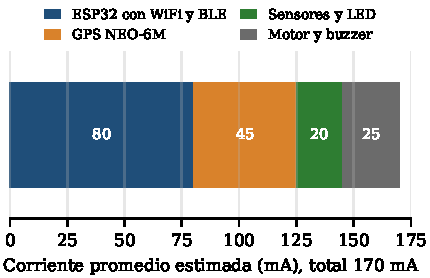
\includegraphics[width=\columnwidth]{resultado_consumo.pdf}
\caption{Consumo promedio estimado por bloque. El ESP32 y el GPS concentran casi tres cuartas partes del total.}
\label{fig:consumo}
\end{figure}

% =====================================================================
\section{Implementación}

\subsection{Lógica de programación}

El firmware está escrito en Arduino IDE con el núcleo ESP32 3.x y las bibliotecas TinyGPSPlus, PubSubClient, ArduinoJson y NimBLE. La Fig.~\ref{fig:flujo} muestra su lógica. El lazo principal no usa \texttt{delay()}. Cada tarea tiene su propio periodo medido con \texttt{millis()}, así ninguna lectura bloquea a las demás. El GPS se revisa en cada vuelta para que no se llene el búfer del puerto serie. El FC-51 se lee cada 10\,ms para no perder el borde de un escalón. La IMU se lee cada 20\,ms, que es lo mínimo para capturar el impacto. La distancia se mide cada 100\,ms porque la función \texttt{pulseIn} puede bloquear hasta 25\,ms. Los actuadores se actualizan cada 50\,ms.

La parte derecha de la figura muestra la máquina de estados. En NORMAL el bastón vibra según la distancia y avisa de desniveles. Una caída confirmada lo lleva a PRE ALERTA, y si nadie pulsa el botón en 10\,s pasa a ALERTA. El pulsador es la única forma de salir de ALERTA, y al hacerlo se publica un mensaje de cancelación para que el tablero borre la alerta. Si el bastón pasa 5 minutos sin moverse entra en REPOSO y apaga los actuadores hasta que vuelva a detectar movimiento.

\begin{figure*}[!t]
\centering
\begin{tikzpicture}[node distance=3.2mm]
  % ---------- Lazo principal ----------
  \node[terminal] (ini) {Inicio};
  \node[proceso, below=of ini] (setup) {Configurar pines, UART2 del GPS, PWM del motor y MPU en $\pm$8\,g};
  \node[proceso, below=of setup] (red) {Iniciar BLE y lanzar la tarea de red en el núcleo 0};
  \node[es, below=of red] (gpsn) {Leer frases NMEA del GPS};
  \node[decision, below=of gpsn] (d10) {¿Pasaron 10\,ms?};
  \node[es, right=5mm of d10] (ir) {Leer FC-51 y evaluar desnivel};
  \node[decision, below=of d10] (d20) {¿Pasaron 20\,ms?};
  \node[es, right=5mm of d20] (imu) {Leer IMU, calcular SVM e inclinación, evaluar caída};
  \node[decision, below=of d20] (d100) {¿Pasaron 100\,ms?};
  \node[es, right=5mm of d100] (dist) {Medir distancia con el HC-SR04};
  \node[decision, below=of d100] (d50) {¿Pasaron 50\,ms?};
  \node[es, right=5mm of d50] (act) {Activar motor y buzzer según el estado};
  \node[proceso, below=of d50] (me) {Actualizar máquina de estados y leer pulsador};

  \draw[flecha] (ini) -- (setup);
  \draw[flecha] (setup) -- (red);
  \draw[flecha] (red) -- (gpsn);
  \draw[flecha] (gpsn) -- (d10);
  \draw[flecha] (d10) -- node[above, font=\tiny]{V} (ir);
  \draw[flecha] (d10) -- node[left, font=\tiny]{F} (d20);
  \draw[flecha] (ir.south) |- ($(d10.south)!0.5!(d20.north)$);
  \draw[flecha] (d20) -- node[above, font=\tiny]{V} (imu);
  \draw[flecha] (d20) -- node[left, font=\tiny]{F} (d100);
  \draw[flecha] (imu.south) |- ($(d20.south)!0.5!(d100.north)$);
  \draw[flecha] (d100) -- node[above, font=\tiny]{V} (dist);
  \draw[flecha] (d100) -- node[left, font=\tiny]{F} (d50);
  \draw[flecha] (dist.south) |- ($(d100.south)!0.5!(d50.north)$);
  \draw[flecha] (d50) -- node[above, font=\tiny]{V} (act);
  \draw[flecha] (d50) -- node[left, font=\tiny]{F} (me);
  \draw[flecha] (act.south) |- ($(d50.south)!0.5!(me.north)$);
  \draw[flecha] (me.west) -- ++(-6mm,0) |- (gpsn.west);
  \node[font=\scriptsize\bfseries, above=1mm of ini] {Lazo principal (núcleo 1)};

  % ---------- Flujo de caída ----------
  \node[es, right=62mm of ini] (c0) {Leer aceleraciones $a_x$, $a_y$, $a_z$ de la IMU};
  \node[decision, below=of c0] (c1) {¿SVM $<$ 0,5\,g?};
  \node[decision, below=of c1] (c2) {¿SVM $>$ 2,5\,g en menos de 1\,s?};
  \node[decision, below=of c2] (c3) {¿Inclinación $>$ 60° por 2\,s?};
  \node[proceso, below=of c3, fill=naranjaclaro] (pre) {PRE ALERTA: vibra 600\,ms de cada segundo};
  \node[decision, below=of pre] (c4) {¿Pulsador antes de 10\,s?};
  \node[alerta, below=of c4] (al) {ALERTA: buzzer intermitente, publica la alerta con GPS por MQTT y BLE};
  \node[decision, below=of al] (c5) {¿Pulsador?};
  \node[es, below=of c5] (canc) {Publicar «cancelada» y volver a NORMAL};

  \node[proceso, right=5mm of c4, text width=17mm] (norm) {Volver a NORMAL};
  \coordinate (descarta) at ($(c1.east)+(14mm,0)$);

  \draw[flecha] (c0) -- (c1);
  \draw[flecha] (c1) -- node[left, font=\tiny]{V} (c2);
  \draw[flecha] (c2) -- node[left, font=\tiny]{V} (c3);
  \draw[flecha] (c3) -- node[left, font=\tiny]{V} (pre);
  \draw[flecha] (pre) -- (c4);
  \draw[flecha] (c4) -- node[above, font=\tiny]{V} (norm);
  \draw[flecha] (c4) -- node[left, font=\tiny]{F} (al);
  \draw[flecha] (al) -- (c5);
  \draw[flecha] (c5) -- node[left, font=\tiny]{V} (canc);
  \draw[flecha] (c5.west) -- node[above, font=\tiny]{F} ++(-5mm,0) |- (al.west);
  \draw[thick] (c1.east) -- node[above, font=\tiny]{F} (descarta);
  \draw[thick] (c2.east) -| node[pos=0.15, above, font=\tiny]{F} (descarta);
  \draw[thick] (c3.east) -| node[pos=0.15, above, font=\tiny]{F} (descarta);
  \draw[flecha] (descarta) |- ($(c0.east)+(0,0)$);
  \node[font=\scriptsize\bfseries, above=1mm of c0] {Detalle de «evaluar caída»};
\end{tikzpicture}
\caption{Diagrama de flujo del firmware. A la izquierda, el lazo principal con tareas periódicas sin bloqueos. A la derecha, el detalle de «evaluar caída» con sus tres fases, la ventana de cancelación y el envío de la alerta. Los paralelogramos son lecturas o salidas, los rectángulos son procesos y cada rombo tiene una salida V (verdadero) y una F (falso).}
\label{fig:flujo}
\end{figure*}

\subsection{Interconexiones entre componentes}

La Fig.~\ref{fig:conexiones} muestra cómo se conecta cada módulo con el ESP32 y la Tabla~\ref{tab:pines} da el mapa de pines definitivo. El FC-51 va en el GPIO 34, que solo sirve como entrada, y se alimenta a 3,3\,V para que su salida no supere el nivel que tolera el ESP32. Hay dos rieles de alimentación. El del pin VIN recibe el voltaje del portapilas y alimenta el HC-SR04, el GPS, el motor y el buzzer. El de 3,3\,V sale del regulador del ESP32 y alimenta el módulo inercial y el FC-51.

\begin{figure*}[!t]
\centering
\begin{tikzpicture}[
  mod/.style={draw, rounded corners=2pt, align=center, font=\scriptsize, text width=23mm, minimum height=9mm, inner sep=2pt},
  pin/.style={font=\tiny, above, align=center, text width=33mm, inner sep=1pt},
  node distance=3mm]
  \node[draw, thick, fill=grisclaro, rounded corners=3pt, minimum width=34mm, minimum height=62mm, align=center, font=\small] (esp) {\textbf{ESP32}\\\textbf{DevKit V1}\\[2mm]\scriptsize regulador\\\scriptsize de 3,3\,V};

  % Izquierda: sensores
  \node[mod, fill=azulclaro, left=36mm of esp.north west, anchor=north east] (hc) {\textbf{HC-SR04}\\pin VIN};
  \node[mod, fill=azulclaro, below=of hc] (mpu) {\textbf{Módulo MPU}\\3,3\,V, I2C 0x68};
  \node[mod, fill=azulclaro, below=of mpu] (fc) {\textbf{FC-51}\\3,3\,V};
  \node[mod, fill=azulclaro, below=of fc] (gps) {\textbf{GPS NEO-6M}\\pin VIN, 9600\,bps};
  \node[mod, fill=azulclaro, below=of gps] (btn) {\textbf{Pulsador}\\a GND};

  \draw[flecha] (hc.east) -- node[pin, pos=0.5]{Trig GPIO 5, Echo GPIO 18\\(Echo por divisor)} (esp.west |- hc.east);
  \draw[doble] (mpu.east) -- node[pin, pos=0.5]{SDA GPIO 21, SCL GPIO 22} (esp.west |- mpu.east);
  \draw[flecha] (fc.east) -- node[pin, pos=0.5]{OUT a GPIO 34} (esp.west |- fc.east);
  \draw[doble] (gps.east) -- node[pin, pos=0.5]{TX a GPIO 16, RX a GPIO 17} (esp.west |- gps.east);
  \draw[flecha] (btn.east) -- node[pin, pos=0.5]{GPIO 27 con pull up} (esp.west |- btn.east);

  % Derecha: actuadores
  \node[mod, fill=naranjaclaro, right=24mm of esp.north east, anchor=north west, text width=46mm] (mot) {\textbf{Módulo vibrador}\\pin VIN, transistor y diodo incluidos};
  \node[mod, fill=yellow!20, below=7mm of mot.south west, anchor=north west, text width=17mm] (q1) {\textbf{Q1} 2N2222\\base 1\,k$\Omega$};
  \node[mod, fill=naranjaclaro, right=6mm of q1] (buz) {\textbf{Buzzer activo}\\pin VIN};

  \draw[flecha] (esp.east |- mot.west) -- node[pin, pos=0.45]{GPIO 25 PWM a IN} (mot.west);
  \draw[flecha] (esp.east |- q1.west) -- node[pin, pos=0.45]{GPIO 26} (q1.west);
  \draw[flecha] (q1) -- (buz);

  % Red
  \node[mod, fill=verdeclaro, below=8mm of q1, text width=17mm] (ble) {\textbf{BLE}\\celular};
  \node[mod, fill=verdeclaro, right=6mm of ble] (wifi) {\textbf{WiFi y MQTT}\\broker y tablero};
  \draw[flecha, verde] (esp.east |- ble.west) -- node[pin, pos=0.45]{antena integrada} (ble.west);
  \draw[flecha, verde] (ble) -- (wifi);

  % Alimentación
  \node[draw, fill=yellow!15, rounded corners=2pt, font=\scriptsize, align=center, text width=60mm, below=7mm of esp] (pwr)
    {\textbf{Alimentación:} portapilas doble (2 $\times$ 3,7\,V en serie) a VIN y GND\\VIN para HC-SR04, GPS, motor y buzzer; 3,3\,V del ESP32 para MPU y FC-51};
  \draw[potencia] (pwr) -- (esp);
\end{tikzpicture}
\caption{Diagrama de interconexiones. Los sensores entran por GPIO, I2C y UART. El módulo vibrador trae su propio driver, y el buzzer se activa con un 2N2222 porque necesita más corriente de la que entrega un pin.}
\label{fig:conexiones}
\end{figure*}

\begin{table}[!t]
\caption{Mapa de pines del ESP32}
\label{tab:pines}
\centering
\footnotesize
\renewcommand{\arraystretch}{1.1}
\begin{tabular}{>{\raggedright\arraybackslash}p{2.6cm} c >{\raggedright\arraybackslash}p{3.6cm}}
\toprule
\textbf{Señal} & \textbf{GPIO} & \textbf{Conexión} \\
\midrule
HC-SR04 Trig y Echo & 5 y 18 & Echo por divisor 1\,k$\Omega$ y 2\,k$\Omega$ \\
MPU SDA y SCL & 21 y 22 & Bus I2C \\
GPS TX y RX & 16 y 17 & UART2 a 9600\,bps \\
FC-51 OUT & 34 & Entrada digital, nivel bajo si ve el piso \\
Portapilas $+$ y $-$ & VIN y GND & Dos celdas de 3,7\,V en serie \\
Pulsador & 27 & Pull up interno, activo en bajo \\
Motor vibrador & 25 & PWM a 5\,kHz, directo a IN del módulo \\
Buzzer & 26 & Salida digital por Q1 \\
\bottomrule
\end{tabular}
\end{table}

\subsection{Comunicación y tablero}

La tarea de red corre en el núcleo 0 y publica en tres tópicos MQTT de un broker público, todos bajo un prefijo propio del grupo. El tópico de estado se publica cada segundo, y al instante cuando cambia el estado o aparece un desnivel, con el estado, la distancia, el desnivel, si el bastón está en uso y el voltaje de la batería. El tópico de alerta se publica al entrar en ALERTA y al cancelar, como mensaje retenido para que un tablero que se conecte tarde vea la última alerta, e incluye latitud, longitud y número de satélites. Si la publicación falla, se reintenta cada segundo. El tópico GPS se publica cada 5\,s, solo cuando hay señal de satélites. Los mismos mensajes JSON se envían por BLE mediante un servicio de tipo UART con notificaciones, al que se conecta el celular.

El tablero web está hecho en HTML y JavaScript. Se conecta al broker por WebSocket seguro, muestra el estado del bastón con mensajes sencillos pensados para la familia y dibuja la posición en un mapa de Leaflet. La Fig.~\ref{fig:tablero} muestra su interfaz: el estado del bastón con la zona de vibración según la distancia, los indicadores de distancia, desnivel, uso y batería, el mapa con la última posición y los mensajes JSON que llegan por MQTT.

\begin{figure}[!t]
\centering
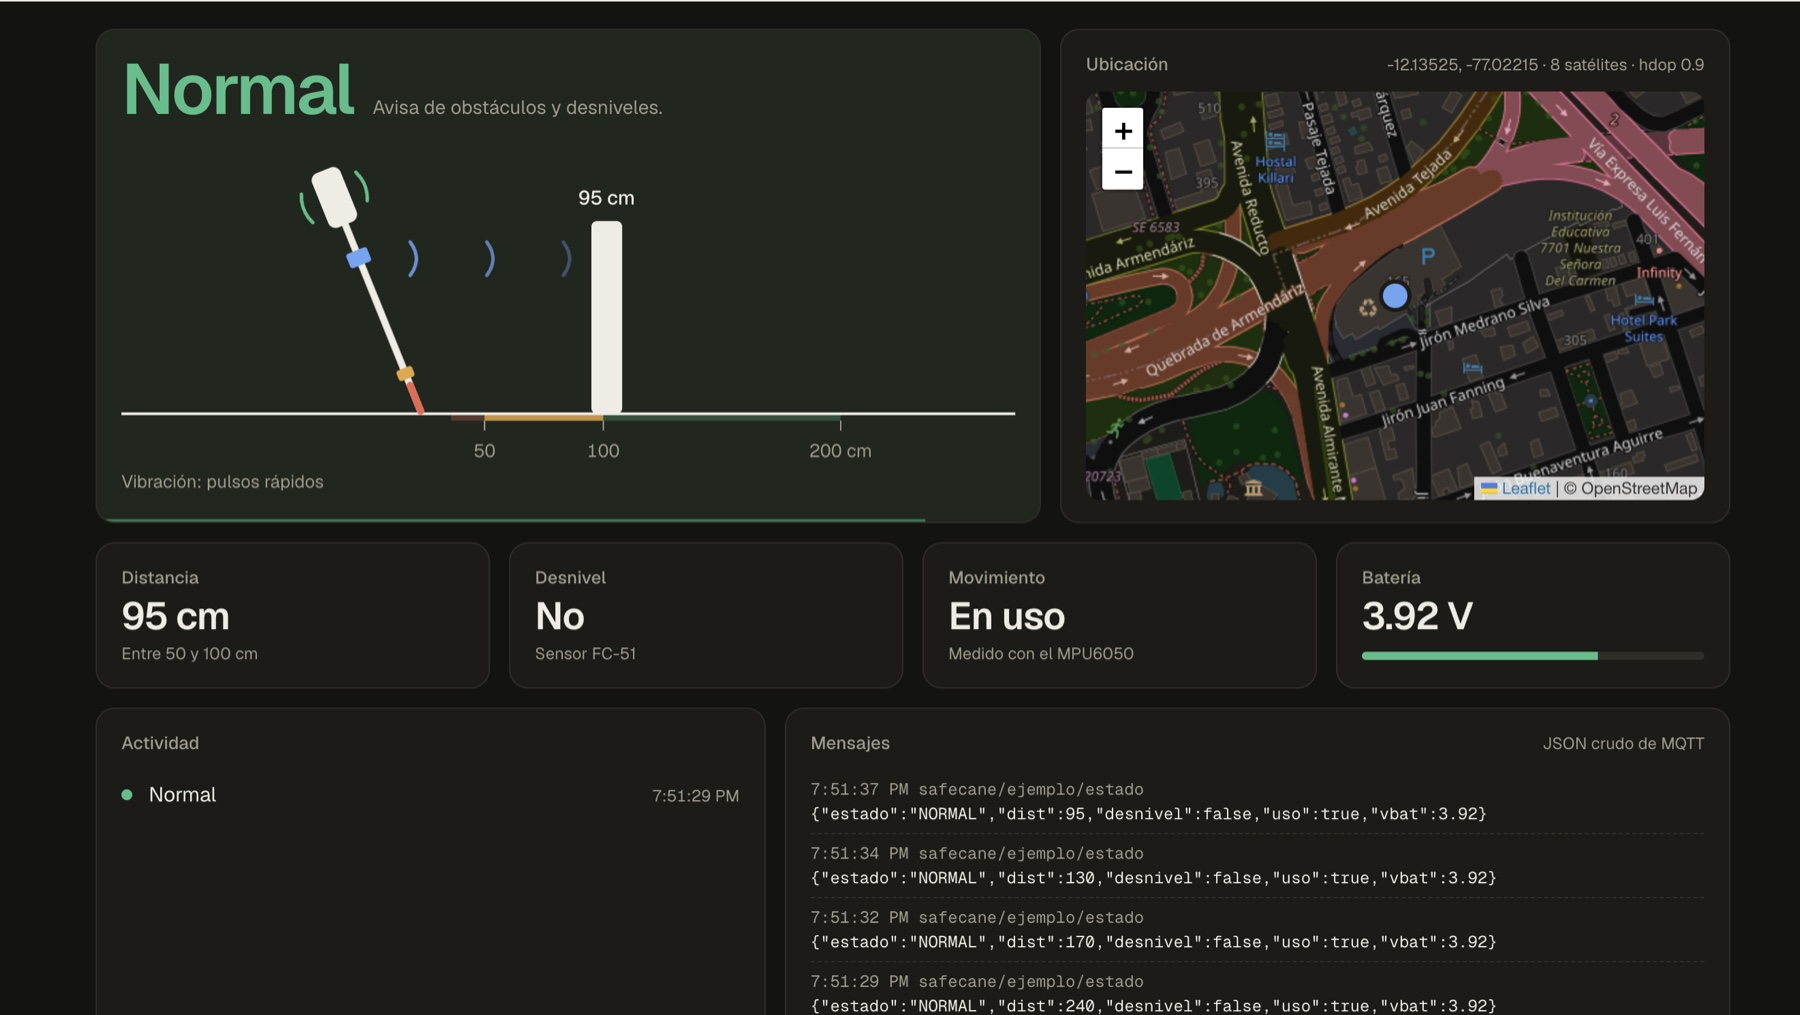
\includegraphics[width=\columnwidth]{captura_tablero.jpg}
\caption{Interfaz del tablero web.}
\label{fig:tablero}
\end{figure}
 Durante las pruebas también usamos un flujo de Node-RED para revisar los mensajes del GPS.

\subsection{Evidencias físicas}

Antes del armado definitivo hicimos una primera integración de todos los módulos en un solo protoboard (Fig.~\ref{fig:integracion}). En esa etapa probamos también una LDR y un LED blanco para la visibilidad nocturna, que no llegaron al prototipo final.

\begin{figure}[!t]
\centering
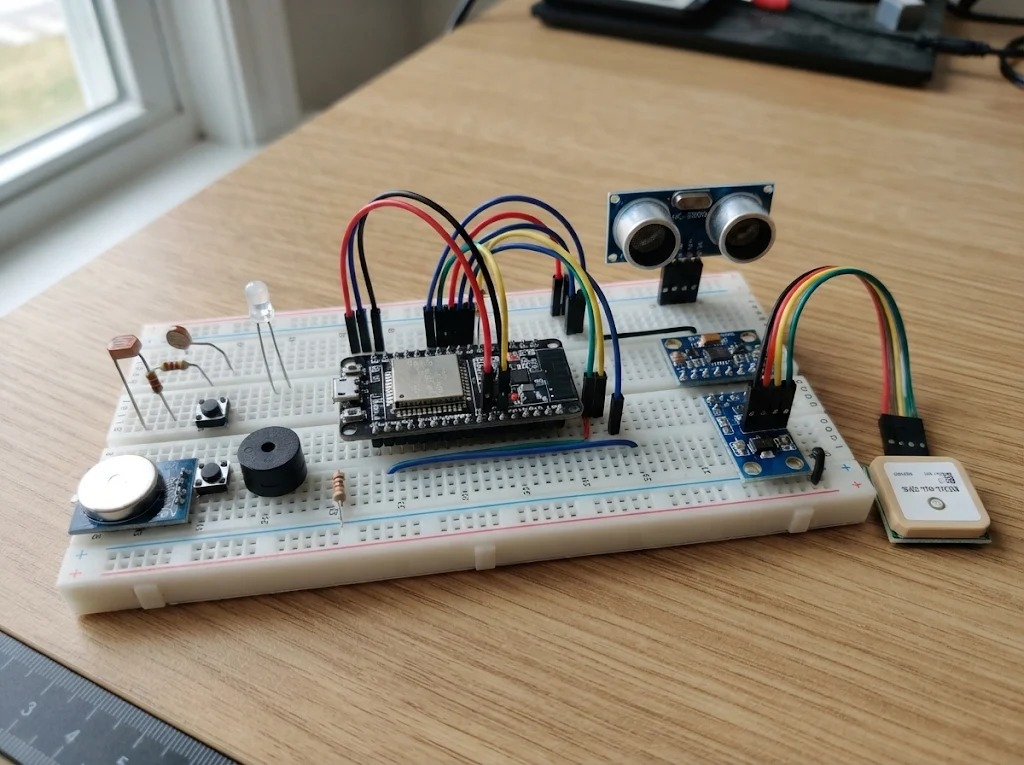
\includegraphics[width=\columnwidth]{foto_primera_integracion.jpg}
\caption{Primera integración en protoboard con el ESP32, el HC-SR04, el módulo inercial, el GPS, el buzzer y el pulsador. La LDR y el LED que se ven a la izquierda no llegaron al prototipo final.}
\label{fig:integracion}
\end{figure}

La Fig.~\ref{fig:armado} muestra el armado del circuito. Primero reunimos los componentes en una mesa de trabajo (Fig.~\ref{fig:armado}a), donde se ven el ESP32 dentro de una caja metálica pequeña, el módulo de carga TP4056, el GPS con su antena cerámica y el primer bastón cubierto con bolsas para proteger la electrónica. Luego montamos todo en dos protoboards unidos (Fig.~\ref{fig:armado}b). Al centro está el ESP32, arriba el módulo del motor vibrador, a la derecha el buzzer y abajo el módulo inercial. La cinta métrica sirvió para medir el espacio que ocupa el circuito, unos 17\,cm de largo. El módulo inercial que conseguimos es una placa de la familia MPU-9250/6500, que comparte con el MPU6050 los registros del acelerómetro que usa el firmware, así que no fue necesario cambiar el código. La energía viene de un portapilas doble con dos celdas de litio de 3,7\,V y 1200\,mAh, cuyo positivo va al pin VIN del ESP32 y su negativo a GND (Fig.~\ref{fig:armado}c). Al poner el portapilas sobre el protoboard medimos un grosor total cercano a 6\,cm (Fig.~\ref{fig:armado}d), y esa medida fijó la altura interna de la caja de control.

\begin{figure*}[!t]
\centering
\begin{subfigure}[b]{0.235\textwidth}\centering
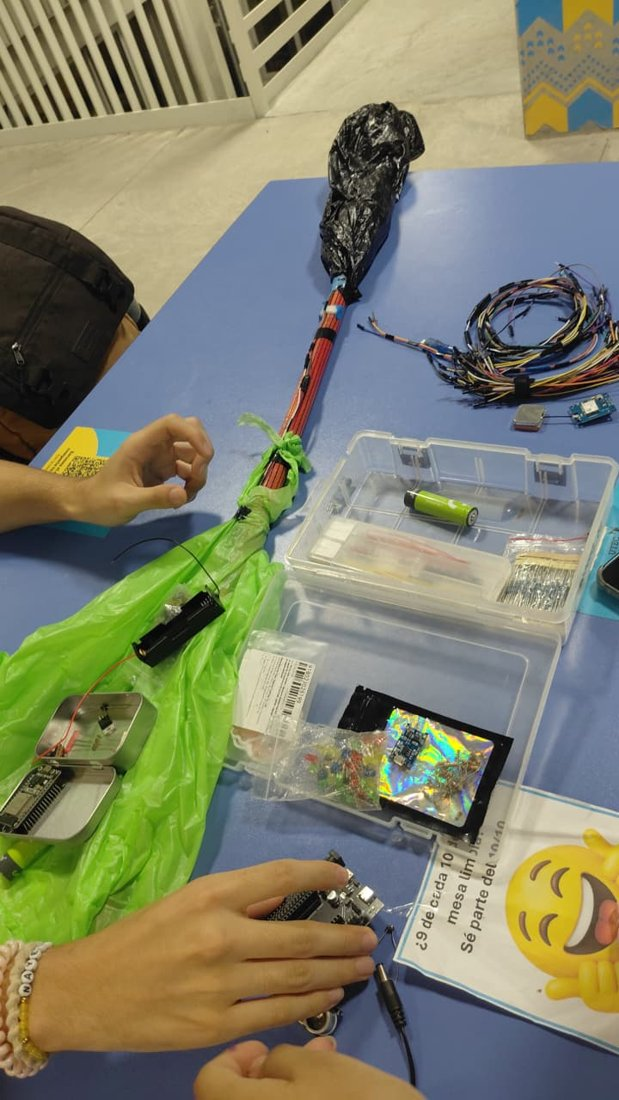
\includegraphics[height=6.4cm]{foto_mesa.jpg}\caption{Componentes en la mesa}
\end{subfigure}\hfill
\begin{subfigure}[b]{0.235\textwidth}\centering
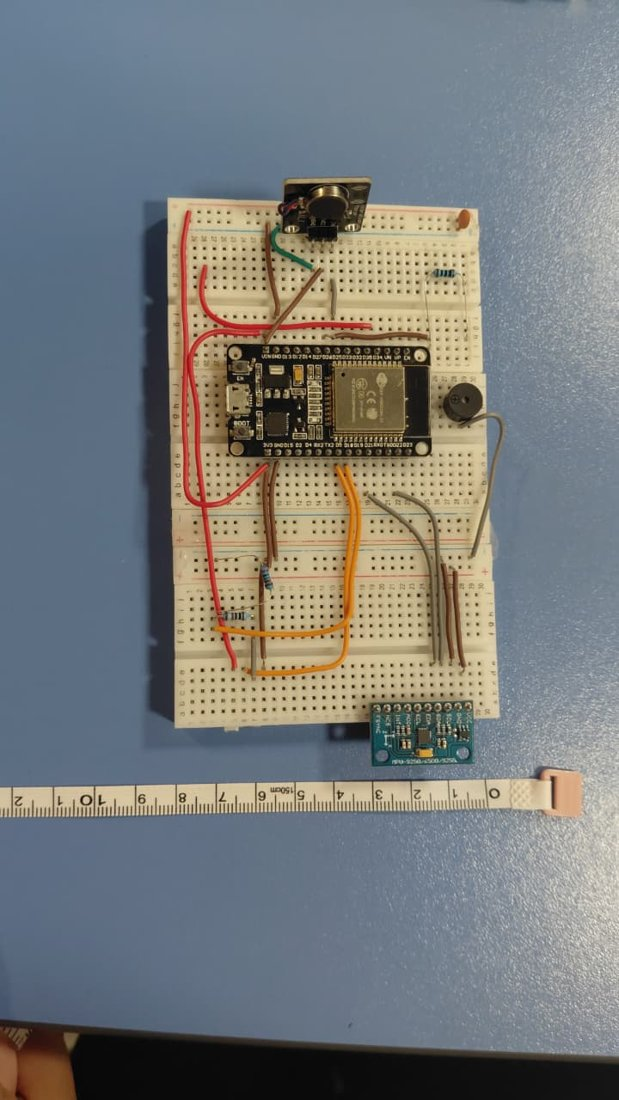
\includegraphics[height=6.4cm]{foto_protoboard.jpg}\caption{Circuito en protoboard}
\end{subfigure}\hfill
\begin{subfigure}[b]{0.235\textwidth}\centering
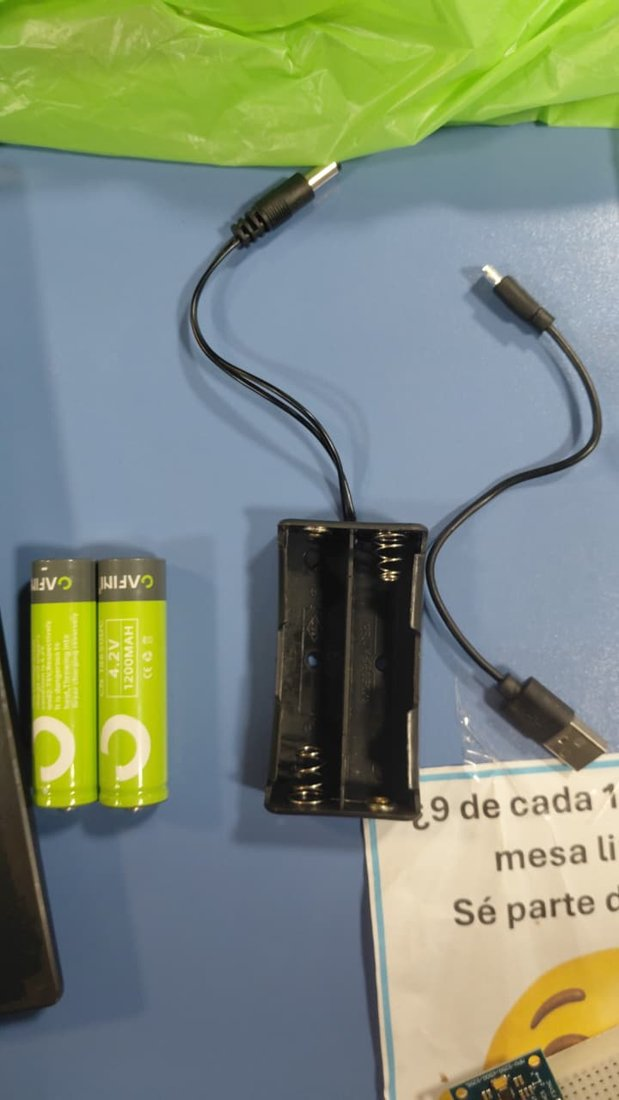
\includegraphics[height=6.4cm]{foto_bateria.jpg}\caption{Portapilas y celdas}
\end{subfigure}\hfill
\begin{subfigure}[b]{0.235\textwidth}\centering
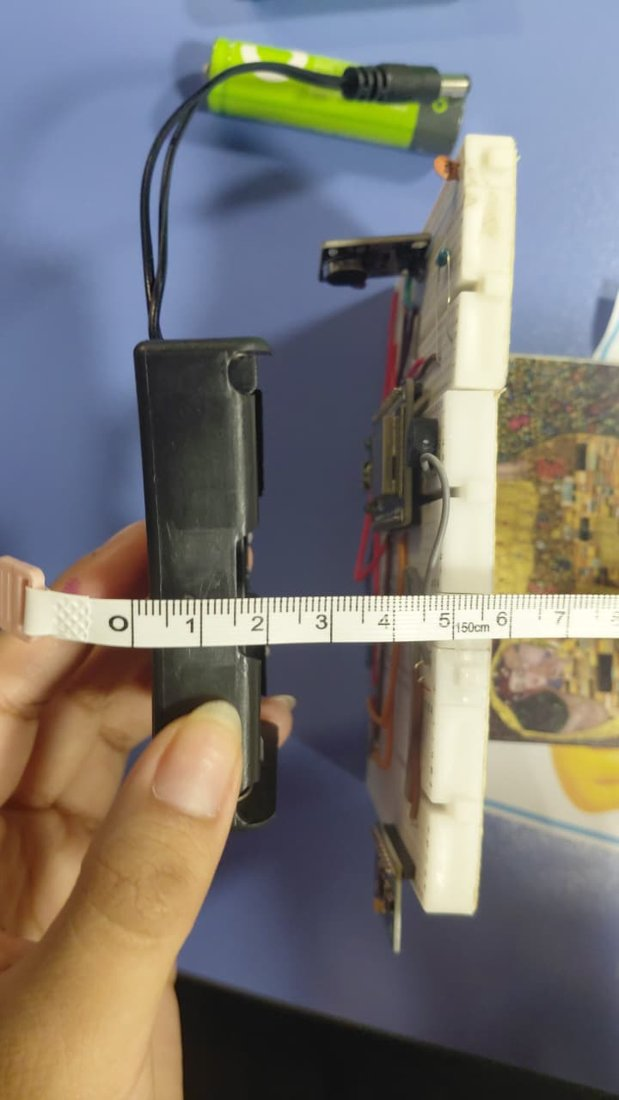
\includegraphics[height=6.4cm]{foto_grosor.jpg}\caption{Grosor del conjunto}
\end{subfigure}
\caption{Armado del circuito de SafeCane: (a) reunión de componentes, (b) integración en protoboard con el ESP32 al centro, (c) alimentación con dos celdas de litio y (d) medición del grosor de batería y protoboard apilados.}
\label{fig:armado}
\end{figure*}

La Fig.~\ref{fig:prototipo}a muestra la versión actual del prototipo, montada sobre un bastón plegable con empuñadura. La caja de control va en la parte superior del tubo, el HC-SR04 está a media altura mirando al frente y el FC-51 va en la punta, protegido con cinta azul. Por ahora la caja es de cartón forrado con cinta, mientras se termina la carcasa definitiva. En su interior (Fig.~\ref{fig:prototipo}b) van los protoboards con el circuito, y de ahí salen los cables hacia los sensores del tubo.

\begin{figure*}[!t]
\centering
\begin{subfigure}[b]{0.40\textwidth}\centering
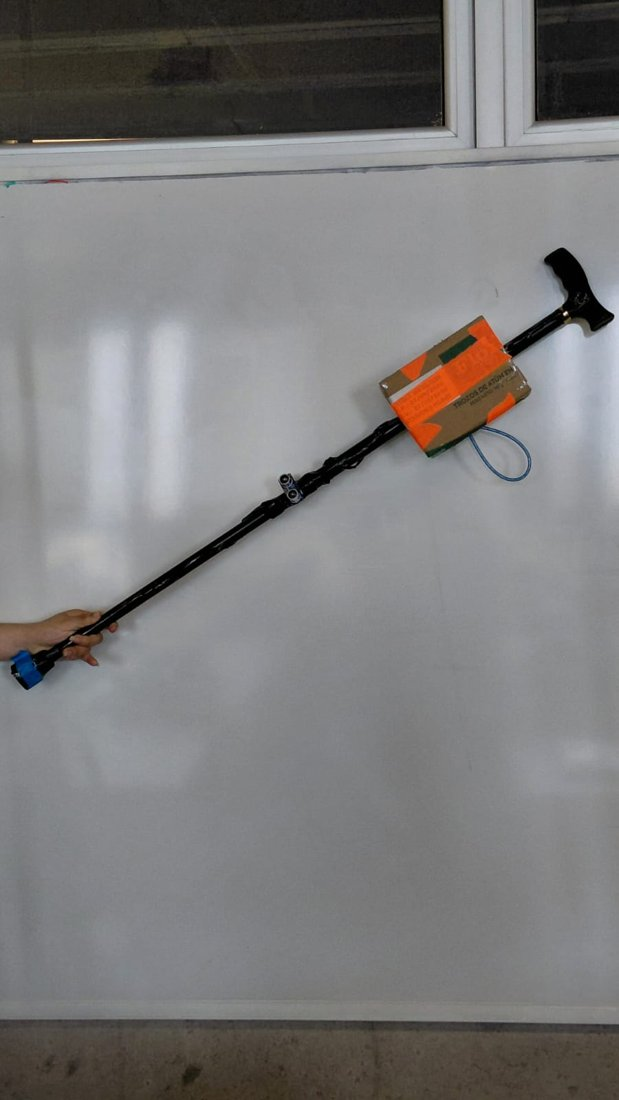
\includegraphics[height=6.4cm]{foto_baston_final.jpg}\caption{Bastón actual}
\end{subfigure}\hspace{8mm}
\begin{subfigure}[b]{0.30\textwidth}\centering
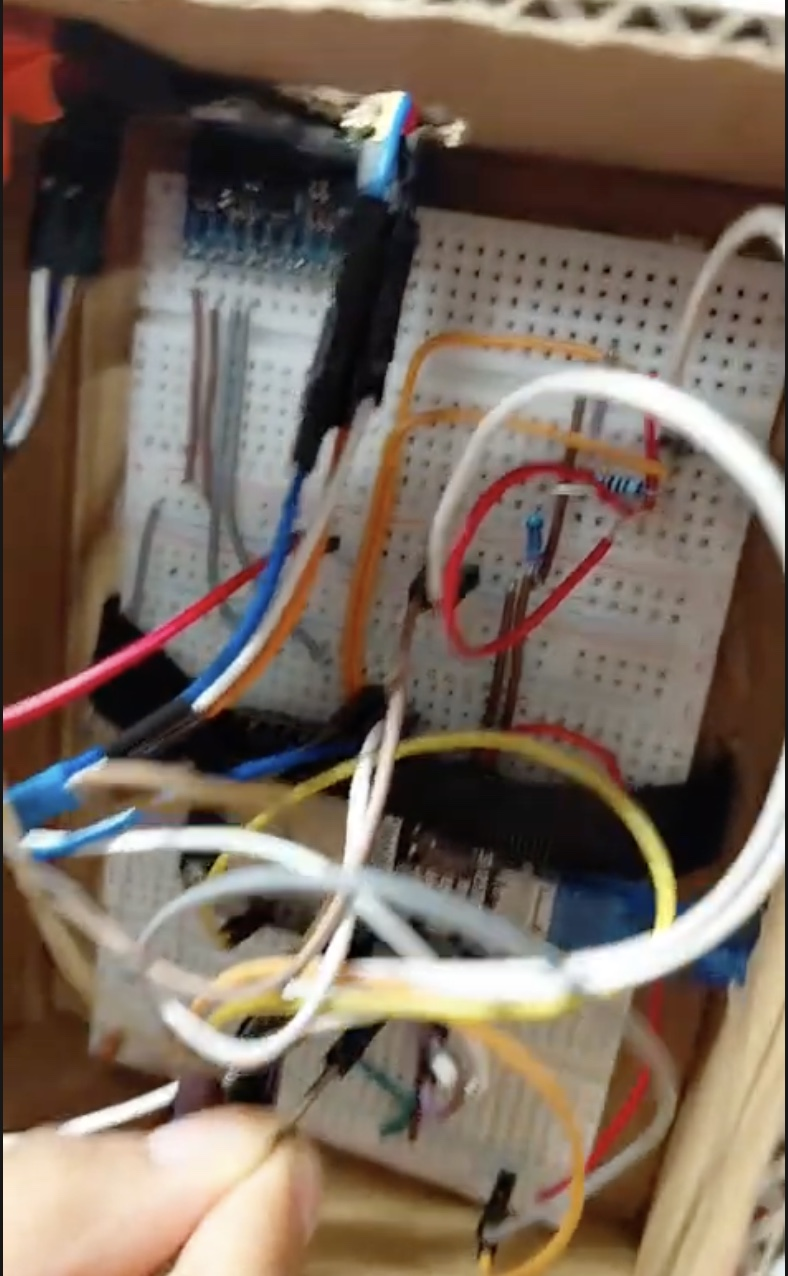
\includegraphics[height=6.4cm]{foto_caja_interior.jpg}\caption{Interior de la caja de control}
\end{subfigure}
\caption{Prototipo actual: (a) bastón plegable con la caja de control, el HC-SR04 a media altura y el FC-51 en la punta, y (b) interior de la caja de cartón con el circuito en protoboard y el cableado hacia los sensores.}
\label{fig:prototipo}
\end{figure*}

La Fig.~\ref{fig:caja} presenta el diseño de la carcasa definitiva. La caja mide 19\,cm por 12\,cm por 7\,cm y por dentro deja 18\,cm por 11\,cm por 6\,cm. La batería va encima del protoboard sobre separadores, el pulsador queda en el frente y el GPS se ubica en la cabeza del bastón para tener mejor vista del cielo.

\begin{figure*}[!t]
\centering
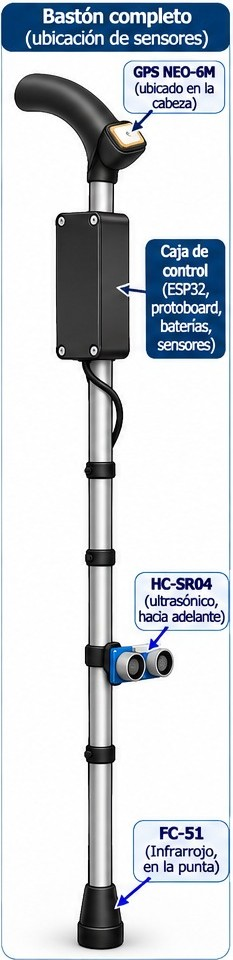
\includegraphics[height=5.3cm]{diseno_baston.jpg}\hspace{3mm}
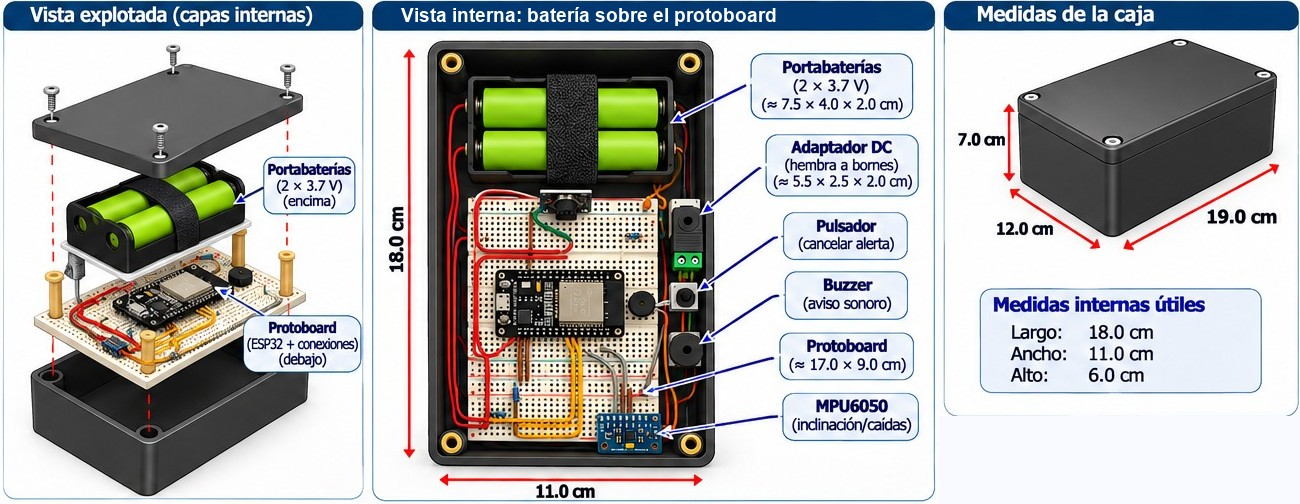
\includegraphics[height=5.3cm]{diseno_caja.jpg}
\caption{Diseño de la carcasa. A la izquierda, la ubicación de los sensores en el bastón. A la derecha, la vista explotada, la distribución interna con las celdas sobre el protoboard y las medidas de la caja.}
\label{fig:caja}
\end{figure*}

% =====================================================================
\section{Análisis de resultados}

\subsection{Verificación del algoritmo de caída}

La Fig.~\ref{fig:caida} es una figura original generada por el equipo. Para obtenerla pasamos a Python la misma lógica de detección del firmware y le aplicamos un perfil de caída sintético: el bastón está vertical, entra en caída libre durante 300\,ms, recibe un impacto durante 100\,ms y queda tumbado. El panel superior muestra la SVM, el del medio la inclinación y el inferior el estado del sistema.

La caída libre empieza en 1,0\,s y la SVM baja a 0,1\,g, por debajo del umbral de 0,5\,g. A los 1,3\,s llega el impacto con 3,46\,g, que supera el umbral de 2,5\,g dentro de la ventana de un segundo. Después la inclinación sube a 90° y se mantiene. El algoritmo espera 0,5\,s a que el bastón se asiente, comprueba la inclinación durante 2\,s y entra en PRE ALERTA a los 3,8\,s. Como nadie cancela, pasa a ALERTA a los 13,8\,s.

Entre el impacto y la alerta remota pasan 12,5\,s, y 10 de ellos corresponden a la ventana de cancelación. Aceptamos esa espera para reducir las falsas alarmas, aunque hay que tenerla en cuenta al comparar con Fitriandini et al. \cite{fitriandini}, cuyo retardo de 4,71\,s no incluye esa espera. Por eso nuestra meta de menos de 5\,s se mide desde que el bastón entra en ALERTA hasta que el mensaje aparece en el tablero. El perfil sintético es ideal: en el bastón real el impacto trae rebotes y la caída libre es más corta, así que los umbrales se deben ajustar con los registros a 50\,Hz de la Fase 4.

\begin{figure}[!t]
\centering
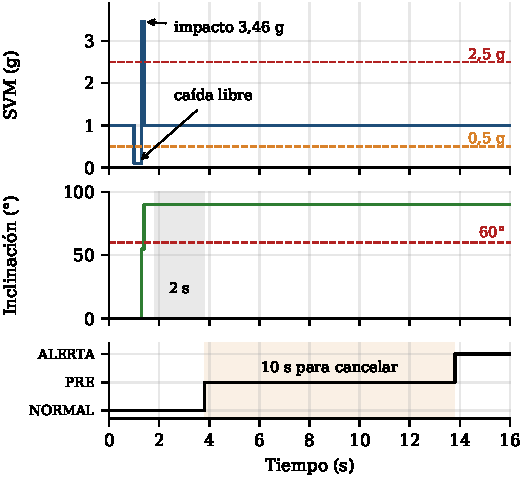
\includegraphics[width=\columnwidth]{resultado_caida.pdf}
\caption{Respuesta del algoritmo de caída al perfil simulado. Se ven las tres fases (caída libre, impacto e inclinación sostenida), la entrada en pre alerta y la alerta tras 10\,s sin cancelar.}
\label{fig:caida}
\end{figure}

\subsection{Respuesta háptica a los obstáculos}

La Fig.~\ref{fig:vibracion}, también original, muestra la intensidad media del motor según la distancia al obstáculo, calculada a partir de los ciclos de trabajo del firmware. Por debajo de 50\,cm el motor vibra al 100\,\%. Entre 50 y 100\,cm pulsa al 78\,\% de su potencia la mitad del tiempo, lo que da una media cercana al 39\,\%. Entre 1 y 2\,m los pulsos son más largos y suaves y la media baja al 24\,\%. Entre la zona rápida y la lenta cambia sobre todo el ritmo, así que el usuario reconoce la cercanía por la frecuencia de los pulsos. El aviso de desnivel usa un ritmo distinto, 100\,ms encendido y 100\,ms apagado junto con el buzzer, para que no se confunda con un obstáculo.

\begin{figure}[!t]
\centering
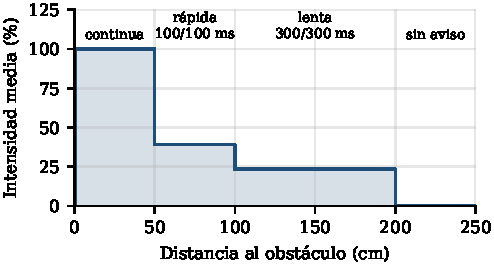
\includegraphics[width=\columnwidth]{resultado_vibracion.pdf}
\caption{Intensidad media del motor vibrador según la distancia al obstáculo, con las tres zonas de aviso del firmware.}
\label{fig:vibracion}
\end{figure}

\subsection{Pruebas con el prototipo}

La Tabla~\ref{tab:resultados} reúne las metas de validación y los resultados de las pruebas con el bastón. Simulamos las caídas sobre colchoneta, solo con integrantes del equipo, y calculamos la sensibilidad como $VP/(VP+FN)$, donde VP son las caídas que el bastón detectó y FN las que dejó pasar.

\begin{table}[!t]
\caption{Metas de validación y resultados}
\label{tab:resultados}
\centering
\footnotesize
\renewcommand{\arraystretch}{1.15}
\begin{tabular}{>{\raggedright\arraybackslash}p{3.1cm} >{\raggedright\arraybackslash}p{1.9cm} p{2.3cm}}
\toprule
\textbf{Métrica} & \textbf{Meta} & \textbf{Resultado} \\
\midrule
Error en distancia & $<$ 3\,cm & 1 a 2\,cm (cumple) \\
Alcance de obstáculos & 2\,m & 4\,m; aviso hasta 2\,m (cumple) \\
Escalones y bordillos detectados & $\geq$ 85\,\% & 90\,\% (cumple) \\
Sensibilidad en caídas & $\geq$ 80\,\% & 80\,\% (cumple) \\
Latencia al tablero & $<$ 5\,s & 5\,s (en el límite) \\
Primer fix del GPS & $<$ 2\,min & 3,5\,min (no cumple) \\
Error de posición GPS & Cerca de 4,63\,m \cite{fitriandini} & $\approx$ 4\,m (cumple) \\
Autonomía real & Estimada 6\,h & 1,5\,h (no cumple) \\
\bottomrule
\end{tabular}
\end{table}

El HC-SR04 midió la distancia con un error de 1 a 2\,cm, dentro de la meta de 3\,cm. El sensor lee hasta unos 4\,m, el límite que fija la espera de 25\,ms de \texttt{pulseIn}, y el firmware hace vibrar el motor por debajo de 2\,m. El FC-51 avisó en el 90\,\% de los pasos por un escalón o bordillo y el algoritmo reconoció el 80\,\% de las caídas simuladas. Para subir esa cifra tenemos que ajustar los umbrales, que tomamos de la literatura, con los registros a 50\,Hz del bastón real. El GPS ubicó el bastón con un error cercano a 4\,m, parecido a los 4,63\,m que reportan Fitriandini et al. \cite{fitriandini}.

La latencia, el primer fix del GPS y la autonomía quedaron en el límite o por debajo de la meta. El tablero tardó unos 5\,s en mostrar los datos nuevos, el mismo periodo con el que el firmware publicaba el estado en esas pruebas. Después cambiamos el firmware para que publique cada segundo y al instante cuando cambia el estado, y nos falta medir de nuevo la latencia. El GPS tardó unos 3,5\,min en dar su primera posición, frente a los 27\,s de arranque en frío que indica el fabricante \cite{neo6m}. Sospechamos que influyen el arranque sin datos de satélites guardados y la parte del cielo que tapan la caja y el cuerpo del usuario.

La batería se agotó en 1,5\,h, la cuarta parte de las 6\,h estimadas. No medimos la corriente real del bastón, así que no sabemos cuánto de la diferencia viene de un consumo mayor a los 170\,mA estimados y cuánto de una capacidad real de las celdas menor que la de su etiqueta.

\subsection{Hallazgos del armado}

Durante el armado nos topamos primero con el espacio. El circuito en protoboard ocupa unos 17\,cm por 9\,cm y con la batería encima llega a casi 6\,cm de alto, así que tuvimos que diseñar una caja más grande de lo previsto. Con una placa perforada o un circuito impreso ese volumen bajaría.

El FC-51 tiene que ir a unos 2 a 4\,cm del piso, y en un bastón plegable sus cables cruzan las articulaciones y quedan expuestos a tirones al plegarlo. En energía, el portapilas duró 1,5\,h, lejos de la jornada completa que nos propusimos. Por último, conviene dejar la red en su propio núcleo desde el inicio: el cliente MQTT puede tardar varios segundos en reintentar la conexión al broker, y esa espera no debe frenar la lectura de los sensores.

% =====================================================================
\section{Descripción del mercado}

El segmento principal son las personas con discapacidad visual y los adultos mayores que caminan solos en ciudades del Perú, un grupo que supera el millón y medio de personas según el INEI \cite{inei}. Quien toma la decisión de compra suele ser la familia o el cuidador, que busca tranquilidad cuando su familiar sale de casa. Un segundo segmento son las instituciones que trabajan con esta población, como centros de rehabilitación, asociaciones de personas con discapacidad, casas de reposo y municipios con programas para el adulto mayor.

Proponemos un modelo de venta del bastón con un precio accesible, basado en componentes comunes del mercado local, y una suscripción mensual opcional para la familia que incluye el tablero web, el historial de alertas y el mapa con la ubicación. Para las instituciones planteamos paquetes de varios bastones con un panel que muestra a todos sus usuarios, junto con capacitación y mantenimiento. El video publicitario del proyecto está disponible en Google Drive:
\begin{center}
\scriptsize\href{https://drive.google.com/drive/folders/11ey5HYlZcAxr-NJHwWC5MyNg1iEe3KnS}{\texttt{drive.google.com/drive/folders/11ey5HYlZcAxr-NJHwWC5MyNg1iEe3KnS}}
\end{center}

% =====================================================================
\section{Conclusiones y recomendaciones}

\subsection{Conclusiones}

Construimos un bastón inteligente que reúne en un solo dispositivo la detección de obstáculos al frente, el aviso de desniveles bajo la punta, la detección de caídas y la ubicación de cada alerta. Ninguno de los trabajos revisados combina esas cuatro funciones, y lo logramos con componentes baratos y fáciles de conseguir en Lima.

Usar el FC-51 para los desniveles fue una buena decisión. Un sensor infrarrojo de bajo costo cubre una zona que el ultrasonido no ve, y la condición del ángulo de uso evita avisos cuando la persona levanta el bastón.

Separar las tareas en los dos núcleos del ESP32 hizo que la alerta local no dependa de la red. Al verificar el algoritmo comprobamos que la detección recorre en orden las tres fases de la caída y que la ventana de cancelación suma 10\,s antes de la alerta remota, a cambio de menos falsas alarmas.

\subsection{Recomendaciones}

Recomendamos completar la calibración de los umbrales de caída con los registros a 50\,Hz del bastón real, porque los valores actuales salen de la literatura y de la simulación. Con esos mismos datos se puede entrenar más adelante un clasificador como el de \cite{shriharini}.

Conviene pasar el circuito a una placa perforada o a un circuito impreso para reducir el tamaño de la caja, y usar un bastón rígido o conectores en las articulaciones del bastón plegable. En la alimentación recomendamos pasar a una celda 18650 de 3000\,mAh con un TP4056 con protección y un elevador MT3608 ajustado a 5,0\,V. Así el HC-SR04, el GPS y el motor reciben los 5\,V para los que están hechos, en lugar del voltaje de las celdas, y la autonomía estimada sube a unas 15\,h. Apagar el GPS mientras no haya alertas la alargaría aún más.

El FC-51 avisa cuando la punta ya llegó al borde del escalón. Para avisar unos 30\,cm antes, una versión futura puede usar un sensor de distancia infrarrojo como el Sharp GP2Y0A21 o uno de tiempo de vuelo como el VL53L0X.

Por último, el broker público no tiene cifrado. Sirve para una demostración, pero un producto real debe usar un broker propio con usuario, contraseña y conexión cifrada, porque la ubicación de una persona es un dato sensible \cite{tsantikidou}.

% =====================================================================
\begin{thebibliography}{99}

\bibitem{atzori}
L. Atzori, A. Iera y G. Morabito, ``The Internet of Things: A survey,'' \emph{Computer Networks}, vol. 54, n.º 15, pp. 2787--2805, 2010, doi: 10.1016/j.comnet.2010.05.010.

\bibitem{tsantikidou}
K. Tsantikidou, G. Delimpaltadakis, D. Diasakos y N. Sklavos, ``AAL-based smart cane system with security and privacy features for blind and visually impaired individuals,'' \emph{Microprocessors and Microsystems}, vols. 114--115, art. 105155, 2025, doi: 10.1016/j.micpro.2025.105155.

\bibitem{dakopoulos}
D. Dakopoulos y N. G. Bourbakis, ``Wearable obstacle avoidance electronic travel aids for blind: A survey,'' \emph{IEEE Transactions on Systems, Man, and Cybernetics, Part C (Applications and Reviews)}, vol. 40, n.º 1, pp. 25--35, 2010, doi: 10.1109/TSMCC.2009.2021255.

\bibitem{oms_vision}
World Health Organization, ``Blindness and vision impairment,'' hoja informativa, 10 de febrero de 2026. [En línea]. Disponible: \url{https://www.who.int/news-room/fact-sheets/detail/blindness-and-visual-impairment}

\bibitem{inei}
Instituto Nacional de Estadística e Informática, \emph{Perfil sociodemográfico de la población con discapacidad, 2017}. Lima, Perú: INEI, 2019.

\bibitem{oms_caidas}
World Health Organization, ``Falls,'' hoja informativa, 21 de octubre de 2026. [En línea]. Disponible: \url{https://www.who.int/news-room/fact-sheets/detail/falls}

\bibitem{legood}
R. Legood, P. Scuffham y C. Cryer, ``Are we blind to injuries in the visually impaired? A review of the literature,'' \emph{Injury Prevention}, vol. 8, n.º 2, pp. 155--160, 2002, doi: 10.1136/ip.8.2.155.

\bibitem{shriharini}
A. Shri Harini, N. Shaji, A. S. Karthick Rajaa y G. Gugapriya, ``MLP powered IoT-enabled smart cane for the visually impaired: Mobility enhancement and fall detection through sensor based behavior analysis,'' en \emph{ICT Analysis and Applications}, Lecture Notes in Networks and Systems, vol. 1656, S. Fong, N. Dey y A. Joshi, Eds. Cham, Suiza: Springer, 2026, pp. 464--473, doi: 10.1007/978-3-032-06703-6\_44.

\bibitem{paredes}
D. L. Paredes Orozco y M. Domínguez-Morales, ``Smart cane for the visually impaired,'' en \emph{Recent Advances and Emerging Challenges in STEM}, Springer Proceedings in Materials, vol. 50, Y. Torres, A. M. Beltrán, M. Félix, E. Peralta y D. F. Larios, Eds. Cham, Suiza: Springer, 2024, pp. 451--460, doi: 10.1007/978-3-031-64106-0\_49.

\bibitem{fitriandini}
L. Fitriandini, S. Suhardi y K. Sari, ``Fall detector pada lansia berbasis IoT menggunakan sensor MPU-6050 dan sensor GPS Neo 6M,'' \emph{Journal of Telecommunication, Electronics and Control Engineering (JTECE)}, vol. 7, n.º 1, pp. 10--22, 2025, doi: 10.20895/jtece.v7i1.1496.

\bibitem{abuelmakarem}
H. S. Abuelmakarem, A. Abuelhaag, M. Raafat y S. Ayman, ``An integrated IoT smart cane for the blind and visually impaired individuals,'' \emph{SVU-International Journal of Engineering Sciences and Applications}, vol. 5, n.º 1, pp. 71--78, 2024, doi: 10.21608/svusrc.2023.222096.1137.

\bibitem{mpu6050}
InvenSense, \emph{MPU-6000 and MPU-6050 Product Specification}, rev. 3.4, 2013.

\bibitem{bourke}
A. K. Bourke, J. V. O'Brien y G. M. Lyons, ``Evaluation of a threshold-based tri-axial accelerometer fall detection algorithm,'' \emph{Gait \& Posture}, vol. 26, n.º 2, pp. 194--199, 2007, doi: 10.1016/j.gaitpost.2006.09.012.

\bibitem{neo6m}
u-blox, \emph{NEO-6 u-blox 6 GPS Modules Data Sheet}, doc. GPS.G6-HW-09005, 2011.

\bibitem{mqtt}
OASIS, \emph{MQTT Version 5.0}, OASIS Standard, 7 de marzo de 2019. [En línea]. Disponible: \url{https://docs.oasis-open.org/mqtt/mqtt/v5.0/os/mqtt-v5.0-os.html}

\bibitem{appiah}
O. Appiah y W. Elmannai, ``A smart cane with fall detection system for people with visual impairments,'' en \emph{2023 IEEE Int. Conf. on Dependable, Autonomic and Secure Computing, Int. Conf. on Pervasive Intelligence and Computing, Int. Conf. on Cloud and Big Data Computing, Int. Conf. on Cyber Science and Technology Congress (DASC/PiCom/CBDCom/CyberSciTech)}, 2023, pp. 1010--1015, doi: 10.1109/DASC/PiCom/CBDCom/Cy59711.2023.10361350.

\bibitem{geng}
H. Geng, X. Hao, Y. Fang, Y. Guo, Y. Lu y D. Liu, ``Intelligent cane fall detection method combining multilevel threshold and interactive confirmation mechanism,'' en \emph{Proc. 4th Int. Conf. on Algorithms, Network, and Communication Technology (ICANCT 2025)}, Proc. SPIE, vol. 14133, 2026, doi: 10.1117/12.3109628.

\bibitem{putera}
D. A. Putera, R. Adi, D. E. Kurniawan, A. M. Leman y R. Raynold, ``Development of an IoT-based smart cane with non-invasive health monitoring for elderly care in Batam,'' \emph{Journal of Applied Informatics and Computing}, vol. 9, n.º 5, pp. 2879--2890, 2025, doi: 10.30871/jaic.v9i5.11107.

\bibitem{esp32}
Espressif Systems, \emph{ESP32 Series Datasheet}, v5.3. [En línea]. Disponible: \url{https://www.espressif.com/sites/default/files/documentation/esp32_datasheet_en.pdf}

\end{thebibliography}

\end{document}
